d) Escribir funciones que permitan determinar:
\newline\hspace*{15mm}
a. La cantidad de nodos de un árbol binario.
\newline\hspace*{15mm}
b. La suma del contenido de todos los nodos en un
árbol binario.
\newline\hspace*{15mm}
c. La profundidad de un árbol binario.
\newline\hspace*{15mm}
d. El número de ocurrencias de un elemento en un
árbol binario.
\lstinputlisting{Arboles/TareaD.c}
Capturas de Pantalla de Arboles/TareaD.c
\newline
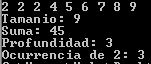
\includegraphics{Arboles/img/TareaD_1.png}
